% Template for ICIP-2018 paper; to be used with:
%          spconf.sty  - ICASSP/ICIP LaTeX style file, and
%          IEEEbib.bst - IEEE bibliography style file.
% --------------------------------------------------------------------------
\documentclass{article}
\usepackage{spconf,amsmath,graphicx}

% Example definitions.
% --------------------
\def\x{{\mathbf x}}
\def\L{{\cal L}}

% Title.
% ------
\title{REAL-TIME TRASHCAN RECOGNIZER AND LOCALIZER FOR THE BLIND AND VISUALLY IMPAIRED}
%
% Single address.
% ---------------
\name{A. Abuyazid, A. Shukla, M. Swaminathan\thanks{Thanks to Dr. Alan C Bovik, Cockrell Family Regents Endowed Chair Professor, The University of Texas at Austin}}
%
% For example:
% ------------
\address{The University of Texas at Austin\\
	Department of Electrical and Computer Engineering\\
	Austin, TX 78712 USA}
%
% Two addresses (uncomment and modify for two-address case).
% ----------------------------------------------------------
%\twoauthors
%  {A. Author-one, B. Author-two\sthanks{Thanks to XYZ agency for funding.}}
%	{School A-B\\
%	Department A-B\\
%	Address A-B}
%  {C. Author-three, D. Author-four\sthanks{The fourth author performed the work
%	while at ...}}
%	{School C-D\\
%	Department C-D\\
%	Address C-D}
%
\begin{document}
%\ninept
%
\maketitle
%
\begin{abstract}
With 324 million people blind and visually impaired in the world and the cane still being the primary assistive device used, we approached this problem by looking at it through a different lens. Quite literally a lens. Through involvement with the National Federation of the Blind, we learned that trivial tasks such as finding a public trash can is almost impossible with merely a cane. Using cameras to help the blind is a pre-existing domain, however, we decided to attack this subproblem of navigating the user to public trash cans. Although seemingly trivial, this concept can be expanded to solve larger, problems such as steering the blind away from hazardous construction, reading signs, and perhaps one day driving (unless self driving cars are prominent by then).
\end{abstract}
%
\begin{keywords}
Image processing, object detection, assistive technology
\end{keywords}
%
\section{INTRODUCTION}
\label{sec:intro}

These guidelines include complete descriptions of the fonts, spacing, and
related information for producing your proceedings manuscripts. Please follow
them and if you have any questions, direct them to Conference Management
Services, Inc.: Phone +1-979-846-6800 or email
to \\\texttt{papers@2018.ieeeicip.org}.


\section{RELATED WORK}
\label{sec:research}

To achieve the best rendering both in printed proceedings and electronic proceedings, we
strongly encourage you to use Times-Roman font.  In addition, this will give
the proceedings a more uniform look.  Use a font that is no smaller than nine
point type throughout the paper, including figure captions.

In nine point type font, capital letters are 2 mm high.  {\bf If you use the
smallest point size, there should be no more than 3.2 lines/cm (8 lines/inch)
vertically.}  This is a minimum spacing; 2.75 lines/cm (7 lines/inch) will make
the paper much more readable.  Larger type sizes require correspondingly larger
vertical spacing.  Please do not double-space your paper.  TrueType or
Postscript Type 1 fonts are preferred.

The first paragraph in each section should not be indented, but all the
following paragraphs within the section should be indented as these paragraphs
demonstrate.

\section{PROCESS}
\label{sec:theprocess}

Major headings, for example, "1. Introduction", should appear in all capital
letters, bold face if possible, centered in the column, with one blank line
before, and one blank line after. Use a period (".") after the heading number,
not a colon.

\subsection{REALSENSE CAMERA}
\label{ssec:realsense}

For this device, we used an Intel Realsense D435 camera to use to detect the trash cans. We chose this because of its relatively small size and since it had two lenses that we could extrapolate depth from. The camera also had depth sensing capabilities, but we chose not to use that and instead use triangulation properties to infer depth because if this device were to become an actual product, the cost of obtaining a camera with depth capabilities are significantly more expensive than using two cameras side by side. The horizontal FOV (field of vision) for the Realsense camera is 86 degrees and the vertical is 57 degrees. We used the librealsense python interface \[\] to capture the individual frames to use for processing. We did not have the capabilities to change the frame of the camera, but we instead modulated the rate at which we sampled the frame in software. 

\subsection{FRAME PRE-PROCESSING}
\label{ssec:frprep}

Ultimately, this device is supposed to be a wearable device, and we kept that in mind as we determined the frame image pre-processing. From training our model, discussed in the model section, we realized that we did not need such a high resolution for the model to work and detect the trash can, so we experimented with downsampling 

\subsection{DATA PRUNING AND CONNECTED COMPONENT LABELING}
\label{ssec:dataprune}

Subheadings should appear in lower case (initial word capitalized) in
boldface.  They should start at the left margin on a separate line.
 
\subsection{THE MODEL}
\label{ssec:themodel}

Subheadings should appear in lower case (initial word capitalized) in
boldface.  They should start at the left margin on a separate line.
 
\subsection{BOOSTING ACCURACY VIA POST TRAINING IMAGE PROCESSING}
\label{ssec:boosting}

Subheadings should appear in lower case (initial word capitalized) in
boldface.  They should start at the left margin on a separate line.
 
\subsection{BINOCULAR CAMERA GEOMETRY AND TRIANGULATION FOR DEPTH APPROXIMATION}
\label{ssec:triangulation}

Subheadings should appear in lower case (initial word capitalized) in
boldface.  They should start at the left margin on a separate line.
 

\subsection{THE DEVICE}
\label{ssec:thedevice}

The device is in the form of a wrist band that contains a 2-dimensional array of haptic motors to relay angular position and distance feedback to the user corresponding to the found trash can. The corresponding LED grid was only for demo purposes so that the audience can view which haptic motors are being activated. We decided on a wrist cuff since the study from the paper, Guiding Blind People with Haptic Feedback, found that the wrist and spine were the best places to detect vibrational impulses \[\]. In their study they used 2 wristbands, but we decided to go with one wristband representing 86 degrees since this was the horizontal FOV (field of vision) of the Intel Realsense camera.

\section{RESULTS}
\label{sec:results}

Use footnotes sparingly (or not at all!) and place them at the bottom of the
column on the page on which they are referenced. Use Times 9-point type,
single-spaced. To help your readers, avoid using footnotes altogether and
include necessary peripheral observations in the text (within parentheses, if
you prefer, as in this sentence).



\section{CONCLUSION}
\label{sec:conclusion}

Print your properly formatted text on high-quality, 8.5 x 11-inch white printer
paper. A4 paper is also acceptable, but please leave the extra 0.5 inch (12 mm)
empty at the BOTTOM of the page and follow the top and left margins as
specified.  If the last page of your paper is only partially filled, arrange
the columns so that they are evenly balanced if possible, rather than having
one long column.

In LaTeX, to start a new column (but not a new page) and help balance the
last-page column lengths, you can use the command ``$\backslash$pagebreak'' as
demonstrated on this page (see the LaTeX source below).

\section{ILLUSTRATIONS, GRAPHS, AND PHOTOGRAPHS}
\label{sec:illust}

Illustrations must appear within the designated margins.  They may span the two
columns.  If possible, position illustrations at the top of columns, rather
than in the middle or at the bottom.  Caption and number every illustration.
All halftone illustrations must be clear black and white prints.  Colors may be
used, but they should be selected so as to be readable when printed on a
black-only printer.

Since there are many ways, often incompatible, of including images (e.g., with
experimental results) in a LaTeX document, below is an example of how to do
this \cite{Lamp86}.

% Below is an example of how to insert images. Delete the ``\vspace'' line,
% uncomment the preceding line ``\centerline...'' and replace ``imageX.ps''
% with a suitable PostScript file name.
% -------------------------------------------------------------------------
\begin{figure}[htb]

\begin{minipage}[b]{1.0\linewidth}
  \centering
  \centerline{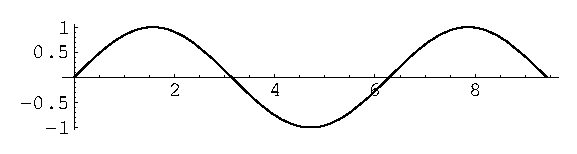
\includegraphics[width=8.5cm]{image1}}
%  \vspace{2.0cm}
  \centerline{(a) Result 1}\medskip
\end{minipage}
%
\begin{minipage}[b]{.48\linewidth}
  \centering
  \centerline{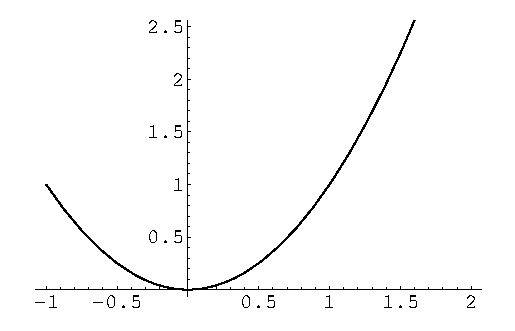
\includegraphics[width=4.0cm]{image3}}
%  \vspace{1.5cm}
  \centerline{(b) Results 3}\medskip
\end{minipage}
\hfill
\begin{minipage}[b]{0.48\linewidth}
  \centering
  \centerline{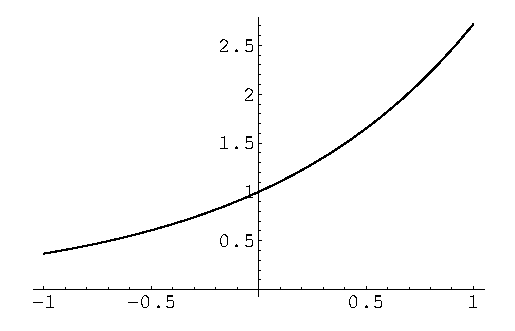
\includegraphics[width=4.0cm]{image4}}
%  \vspace{1.5cm}
  \centerline{(c) Result 4}\medskip
\end{minipage}
%
\caption{Example of placing a figure with experimental results.}
\label{fig:res}
%
\end{figure}


% To start a new column (but not a new page) and help balance the last-page
% column length use \vfill\pagebreak.
% -------------------------------------------------------------------------
%\vfill
%\pagebreak


% References should be produced using the bibtex program from suitable
% BiBTeX files (here: strings, refs, manuals). The IEEEbib.bst bibliography
% style file from IEEE produces unsorted bibliography list.
% -------------------------------------------------------------------------
\bibliographystyle{IEEEbib}
\bibliography{strings,refs}

\end{document}
